% =========================================================================
% KSTAR CES 10 ms gap filling -- 8-page CVPR-style paper (the only paper version).
% Numbers traced to THESIS_RESULTS.md §0 and the sections it cites (2026-11-11),
% plus the review-loop round-1 analyses (2026-11-13): A1 V_rot fit-failure rule
% (docs/paper/vrot_failfit_sensitivity.json), A2 decomposition
% (docs/paper/b28_decomposition.json), A3 noise-corrected coupling bound
% (docs/paper/fast_target_coupling_bound.json).
% Per-split values not printed in the record are read from the artifacts it names:
% docs/paper/paper_numbers.json (RMSE ladder, per-split headline CIs, ablation means,
% MNAR, test shot counts), docs/paper/b27_kfold_interval_R10.json (fold-level column),
% docs/paper/b27c_hier.json (pooled column), docs/b28_weight_physics_report.md
% (forget-gate readout of the 30 frozen checkpoints).
% Build (from this folder): latexmk -pdf main_short
% =========================================================================
\documentclass[10pt,twocolumn,letterpaper]{article}

\usepackage[textwidth=6.875in,textheight=8.875in,columnsep=0.3125in,
            top=1in,headheight=0pt,headsep=0pt,centering]{geometry}
\usepackage[T1]{fontenc}
\usepackage[utf8]{inputenc}
\usepackage{newtxtext,newtxmath}
\usepackage{amsmath,bm}
\usepackage{graphicx}
\usepackage{booktabs}
\usepackage{multirow}
\usepackage{microtype}
\usepackage[compact]{titlesec}
\usepackage[numbers,sort&compress]{natbib}
\usepackage[colorlinks=true,linkcolor=blue,citecolor=blue,urlcolor=blue]{hyperref}

\titleformat{\section}{\normalfont\large\bfseries}{\thesection.}{0.5em}{}
\titleformat{\subsection}{\normalfont\normalsize\bfseries}{\thesubsection.}{0.5em}{}
\titlespacing*{\section}{0pt}{8pt plus 2pt minus 2pt}{4pt plus 1pt}
\titlespacing*{\subsection}{0pt}{6pt plus 2pt minus 1pt}{3pt plus 1pt}
\renewcommand{\bibfont}{\small}
\setlength{\bibsep}{1pt plus 0.5pt}
\setlength{\abovecaptionskip}{4pt}
\setlength{\belowcaptionskip}{0pt}
\setlength{\textfloatsep}{8pt plus 2pt minus 2pt}
\setlength{\floatsep}{6pt plus 2pt minus 2pt}
\setlength{\dbltextfloatsep}{8pt plus 2pt minus 2pt}

\newcommand{\Ti}{\ensuremath{T_i}}
\newcommand{\Vrot}{\ensuremath{V_\mathrm{rot}}}
\newcommand{\skillp}{\ensuremath{\mathrm{skill}_{\mathrm{PCHIP}}}}
\newcommand{\seqv}{\texttt{seq\_v2}}

\graphicspath{{../figures/}}

\hypersetup{
  pdftitle={Filling 10 ms Charge-Exchange Spectroscopy Gaps in KSTAR: What Co-located Fast Diagnostics Add to the Ion-Temperature Past, and a Bound for Rotation},
  pdfauthor={Seungsang Lee},
}

\title{\vspace{-0.3in}\large\textbf{Filling 10\,ms Charge-Exchange Spectroscopy Gaps in KSTAR:
What Co-located Fast Diagnostics Add to the Ion-Temperature Past,
and a Bound for Rotation}}
\author{Seungsang Lee\\
  {\small Department of Nuclear Engineering, Seoul National University}\quad
  {\small\texttt{lss010330@snu.ac.kr}}}
\date{\vspace{-0.25in}}

\begin{document}
\maketitle

% =========================================================================
\begin{abstract}
Charge-exchange spectroscopy (CES) gives KSTAR's ion temperature \Ti{} and toroidal
rotation \Vrot{} at one chord ($R = 2.198$\,m); on the 10\,ms grid of 641 discharges of
the 2022 campaign, 8.2\% of \Ti{} and 23.9\% of \Vrot{} samples are missing. We ask what
beam-emission spectroscopy (BES) and electron-cyclotron-emission imaging (ECEI) channels
within 1.5\,cm of that chord add to the CES past when a step must be filled without the
next CES measurement. A two-branch LSTM reads the fast channels (standardized with each
discharge's own statistics, an offline step) and the CES past for \Ti{}, and only the
CES past for \Vrot{}. For \Ti{}, the mean-squared-error skill of this full-input causal
estimator over a CES-only causal Gaussian-process (GP) smoother is $+0.113$
$[+0.085, +0.132]$ (cut; 95\% interval, eight re-partitions of 639 discharges; the
inclusive interval also excludes zero); the fast-channel share of it is not isolated.
Over PCHIP interpolation the skill is $+0.221$ $[+0.188, +0.248]$, about half of which
a running mean of past CES already provides; against an offline GP it is $-0.010$
$[-0.043, +0.014]$. The gain sits in the tail: the median absolute error (47.2\,eV) is
close to persistence's (46.1\,eV) and above PCHIP's (39.4\,eV; median-AE skill $-0.198$
$[-0.259, -0.135]$). A 20-parameter surrogate filter summarizes the \Ti{} branch post
hoc. For \Vrot{}, the noise-corrected correlation of fast-channel and \Vrot{} increments
is bounded by $|r| \leq 0.044$ (lags 0--200\,ms, windows 10--200\,ms; the \Ti{} lower
bound is at least $+0.127$ at lag 0 for every window). The history-only \Vrot{} estimate has
skill $+0.265$ $[+0.198, +0.326]$ over persistence under a rule set in review that
drops the 0.05\% of rows whose target or anchor exceeds 1{,}000\,km/s; its margin over
the causal GP holds in a pooled readout only, and a margin over PCHIP is not
established. A causally standardized variant is untested. One device, one campaign, one
chord.
\end{abstract}

% =========================================================================
\section{Introduction}
\label{sec:intro}

Ion temperature \Ti{} and toroidal rotation \Vrot{} are core kinetic quantities of a
tokamak plasma; here both come from one outboard chord at $R = 2.198$\,m, with $r/a$
not mapped. Both are measured by charge-exchange
spectroscopy (CES)~\citep{Ko2010ChargeExchange}, which infers \Ti{} from Doppler
broadening and \Vrot{} from the Doppler shift of the charge-exchange line. CES must
integrate photons, so it is slow and intermittently missing: on the KSTAR 10\,ms grid,
8.2\% of \Ti{} and 23.9\% of \Vrot{} observations are missing---independently of each
other---and a further 41.1\% of \Vrot{} rows repeat the previous reading
bit-for-bit, so only 35.0\% of the grid carries an independent \Vrot{} measurement.
The missing rate rises from 0.77\% to 4.45\% across quintiles of neighbouring-step
change and is 19.9\% in the lowest BES-intensity quintile against 3.7\% in the highest,
i.e.\ it is missing-not-at-random~\citep{Little2002StatisticalAnalysis}. Meanwhile
beam-emission spectroscopy (BES), electron-cyclotron-emission imaging (ECEI) and
Mirnov coils observe the same plasma without gaps, but none measures \Ti{} or \Vrot{}.
We ask: \emph{at a 10\,ms step where CES is missing, what do the simultaneous fast
diagnostics add to the irregular CES past?} The use case is an estimate that cannot
wait for the next CES exposure, with fast channels standardized per discharge (offline);
a causally standardized variant is untested under this protocol. Against an offline
noise-aware smoother that reads both neighbours, the skill interval includes zero
(\S\ref{sec:res:headline}).

\paragraph{Comparators.}
Deployable comparators read only the CES past: persistence, a running mean, and a causal
Gaussian process (GP) on the 16 past CES values. Linear and
PCHIP~\citep{fritsch1980} interpolation and an offline GP read both neighbours and serve
as offline references. PCHIP passes exactly through noisy anchors, so a smoother of the
CES past alone already gains on it (running mean $+0.05$ to $+0.17$ over PCHIP, cut,
interval excluding zero on 3/4 splits); the deciding deployable comparison is therefore
the causal GP.

Every result is reported in two co-primary populations: \emph{cut}, in which the
0.53\% of \Ti{} rows above 3\,keV (spectral-fit failures) are treated as missing in
every arm, and \emph{inclusive}, in which they are kept (\S\ref{sec:data}); the
inclusive population's extra margin is mostly spike handling.

\paragraph{Claims.}
\emph{(1) Ion temperature.} The full-input causal estimator exceeds the CES-only causal
GP by $+0.113$ $[+0.085, +0.132]$ (cut; $+0.118$ $[+0.076, +0.157]$ inclusive); the
fast-channel share is not isolated by a retrained history-only model.
\emph{(2) Rotation.} The same channels' noise-corrected correlation with \Vrot{}
increments is bounded by $|r| \leq 0.044$ at 10--200\,ms. \Vrot{} is estimated from its
own history: skill over persistence, a copy-last baseline, $+0.265$
$[+0.198, +0.326]$ (cut, under the fit-failure rule set in review); over the causal GP
$+0.151$ $[+0.038, +0.290]$ pooled, per split 1/4 (cut). Its median row is worse than
persistence (4.3 vs.\ 3.7\,km/s), and its 10\,ms scatter is consistent with Gaussian
line-fit errors ($\sqrt2$ ratio; $\sqrt{T_i}$ scaling not observed).
The evaluation (two co-primary populations, a shot-clustered paired bootstrap, an
overlap-corrected repeated cross-validation interval and a two-level bootstrap,
\S\ref{sec:eval}) is assembled from standard pieces and is described as method, not
claimed. Code and evaluation artifacts are released; the KSTAR shot files are not
redistributable.

% =========================================================================
\section{Related work}
\label{sec:related}

\paragraph{Gap filling and baselines.} GP regression~\citep{rasmussen2006} is the
standard tool for fusion profile fitting~\citep{chilenski2015,michoski2024}, applied
to KSTAR CES \Ti{} profiles~\citep{Kim2024KineticProfile}; PCHIP~\citep{fritsch1980}
avoids spline ringing at steps. We score with Murphy's skill~\citep{murphy1988}.
Persistence as a reference has precedent in fusion profile
forecasting~\citep{Abbate2025Combining} and space weather~\citep{Owens2013Persistence}.

\paragraph{Neural diagnostic inference.} NN-CES extracts \Ti{} and rotation from
KSTAR CES spectra without beam modulation~\citep{Lee2026NeuralNetworkbased}; it is the
closest prior work. Rows with no CES exposure belong to this work; rows with an
existing spectrum but a rejected fit belong to spectral re-analysis such as NN-CES. The
files do not record which case applies, so the split between the two is not measured;
per-exposure fit metadata would resolve it and would replace the value cut. Lin et
al.~\citep{Lin2024PredictionPlasma} map an x-ray crystal spectrometer to \Ti{} and
rotation on EAST, an instantaneous mapping from the same photon channel.
RTCAKENN~\citep{Shousha2023MachineLearningbased} reconstructs kinetic profiles in real
time and tolerates dropped Thomson/CER inputs; there missingness is a robustness
condition, here the target's own sparsity is the problem.

\paragraph{Cross-diagnostic reconstruction.} Diag2Diag synthesizes Thomson
$T_e$/$n_e$ from simultaneous diagnostics on
DIII-D~\citep{Jalalvand2025MultimodalSuperresolution} with a memory-less MLP;
related work densifies Thomson on COMPASS~\citep{Imrek2026TemporalSuperresolution},
fills Thomson intervals causally with an extended Kalman filter on
TCV~\citep{Pastore2023ModelBased}, restores EAST $T_e$ and
$Z_\mathrm{eff}$~\citep{Wang2025TimeSeries,Jia2026TimeSeries} and masks channels on
HL-3~\citep{Yang2026FusionmaeSelfsupervised}. These target electron or generic dense
channels; we extend the programme to a sparse ion channel, to estimation conditioned on
the target's own irregular past, and to per-target tests against pre-registered
baselines.

\paragraph{Methods lineage.} Observation masks follow
GRU-D~\citep{Che2018RecurrentNeural}; the overlap-corrected interval
is~\citep{Nadeau2003Inference}, the repeat-then-discharge resampling is a hierarchical
bootstrap~\citep{Saravanan2020Hierarchical}, and the surrogate retention test follows
the fixed-point readout of~\citep{Maheswaranathan2020HowRecurrent}.

% =========================================================================
\section{Data and problem}
\label{sec:data}

We use 641 KSTAR discharge files (shots 30801--32751) aligned to a 10\,ms grid,
247{,}207 rows in total. Each row holds BES~\citep{Nam2012AnalysisEdge} (9 channels),
ECEI~\citep{Yun2010DevelopmentKstar} (4), Mirnov coils (2), time, and the two CES
targets. \Ti{} is missing in 8.2\% of rows and \Vrot{} in 23.9\%, independently, so
the loss is masked per target (Fig.~\ref{fig:missing}). Both CES targets are the 2022
channel at $R = 2.198$\,m; the nine BES and four ECEI channels lie within about
1.5\,cm of it, and the two Mirnov inputs are two positions of one poloidal array at one
toroidal location. Rows group into contiguous segments at gaps $\geq 0.5$\,s; no arm
bridges a gap.

\paragraph{Held \Vrot{} values.} 54\% of observed \Vrot{} values are bit-identical
repeats of the previous observation (runs up to 1{,}214 rows, 499/641 files); the files
do not record why; the \Ti{} and \Vrot{} masks agree on 72.8\% of rows, so the two
channels are post-processed separately. \Ti{} has 1 held row in 226{,}991.
Holds are removed \emph{everywhere}---targets, history inputs, normalization
statistics and every baseline's anchors---so no arm scores a forward-fill for free.

\paragraph{Fit failures and two populations.} \textbf{1{,}197 \Ti{} rows (0.53\%)
exceed 3\,keV} (951 runs in 274 discharges, 85\% of runs single rows), failed spectral fits
that also poison interpolation anchors. We pre-registered \textbf{two co-primary
populations}: \emph{cut} ($>$3\,keV treated as missing in every arm) and
\emph{inclusive} (no cut); a claim is stated without qualification only if it holds in
both. The threshold is immaterial across 2.5--4\,keV (mean \Ti{} skill $+0.230$ and
$+0.232$ against $+0.236$ at 3\,keV).

\begin{figure}[t]
  \centering
  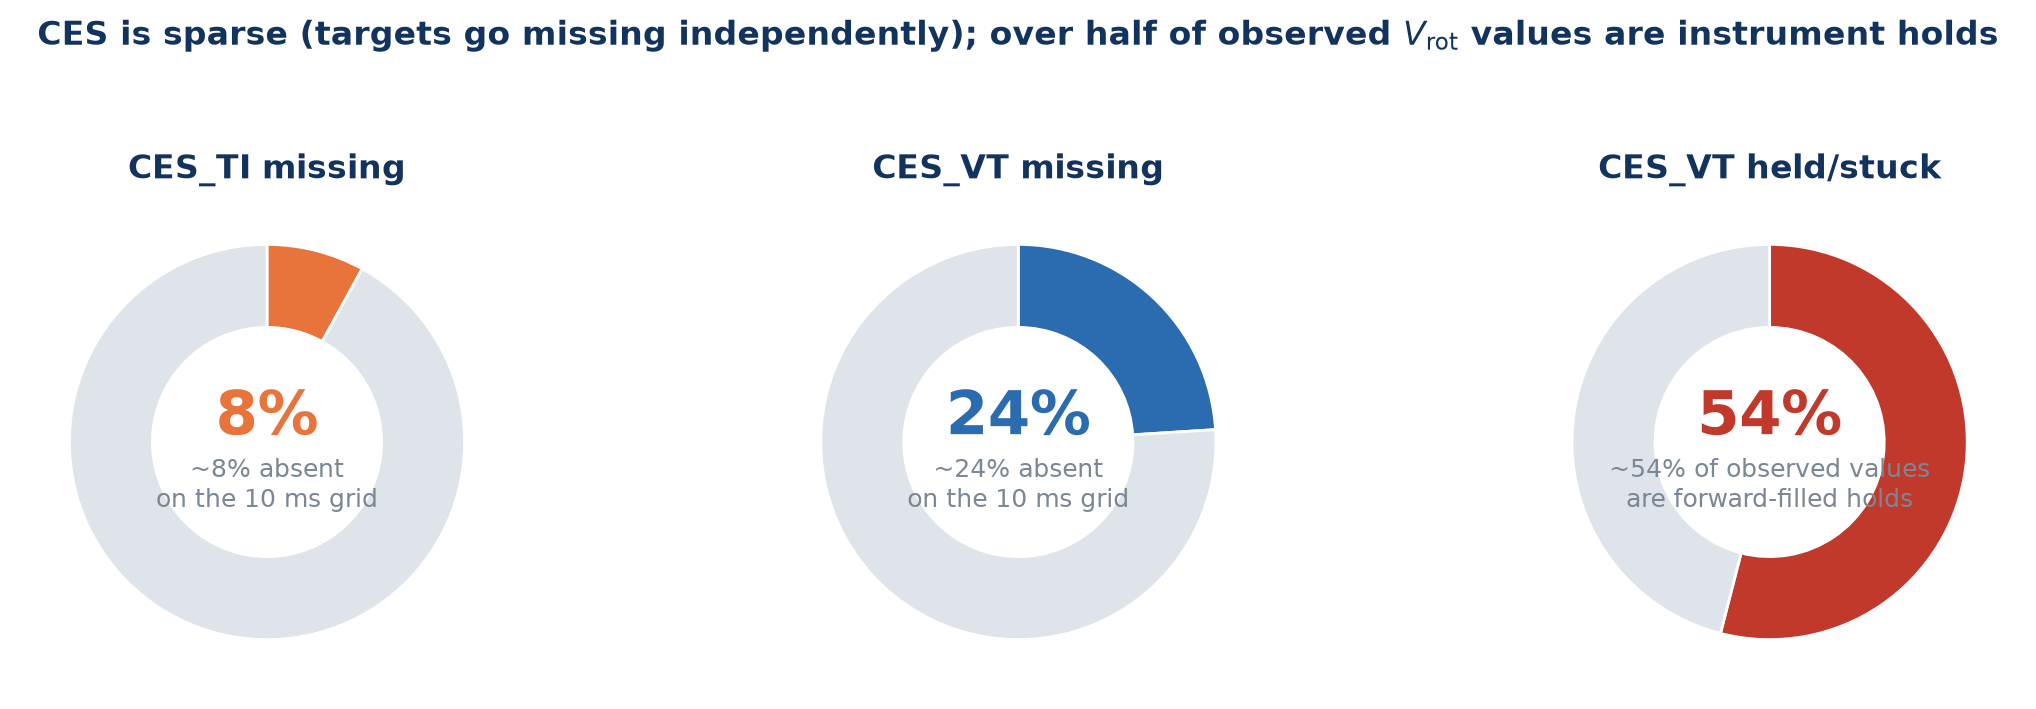
\includegraphics[width=0.92\linewidth]{fig_missing}
  \caption{CES missingness on the 10\,ms grid. \Ti{} and \Vrot{} go missing
  independently (8.2\% / 23.9\%); counting holds, 65.0\% of the grid carries no
  independent \Vrot{} information.}
  \label{fig:missing}
\end{figure}

% =========================================================================
\section{Model}
\label{sec:model}

The main model, \seqv{}, is a 357{,}570-parameter sequence nowcaster. This
section fixes what is estimated, why the inputs are wired to each target, which time
scales the model sits on, and a 20-parameter surrogate of its \Ti{} branch.

\subsection{Estimand, loss and an irreducible floor}
\label{sec:model:target}
At grid time $t$ the model estimates the normalized $y_t=[\Ti,\Vrot]_t$ from
$x_{\le t}$ with per-target observation masks $m_{t,c}\in\{0,1\}$:
\begin{multline}
  \mathcal{L}
  = \frac{\sum_{t,c} m_{t,c}\,(\hat y_{t,c}-y_{t,c})^2}{\sum_{t,c} m_{t,c}}\\
  + \lambda\,\overline{\mathrm{ReLU}(z_0-\hat y_{t,\Ti})},\qquad \lambda = 0.1,
  \label{eq:loss}
\end{multline}
whose first-term minimizer is $\mathbb{E}[y_t\mid x_{\le t}]$; the second term
discourages \Ti{} below the normalized zero $z_0$. A row with one observed target
still supervises it (a both-required filter would discard $\approx$28\% of labelled
rows). The target is itself a photon-integrated fit with noise $\sigma_\mathrm{meas}$,
so even a perfect physical estimate scores
$\mathrm{RMSE}^2=\sigma_\mathrm{meas}^2+b^2$. Difference estimators put
$\sigma_\mathrm{meas}$ for \Ti{} (cut) at 46.4--129.9\,eV, the order of the backbone's
157.8\,eV, and 46.6\% of the fourth-difference squared mass (65.6\% for \Vrot{}) sits
in the top 1\% of one-step changes: \eqref{eq:loss} is a \emph{tail statistic}
(\S\ref{sec:res:dual}).

\subsection{Two conservation laws and the input routing}
\label{sec:model:physics}
Ion energy and toroidal angular momentum obey
\begin{align}
  \partial_t\bigl(\tfrac{3}{2}n_i T_i\bigr) + \nabla\!\cdot\!\mathbf{q}_i
    &= Q_{ei}\,(T_e-T_i) + S_i,
  \label{eq:energy}\\
  \partial_t\bigl(n_i m_i \langle R^2\rangle \omega_\varphi\bigr)
    + \nabla\!\cdot\!\Pi_\varphi
    &= T_\mathrm{NBI} + T_\mathrm{NTV} + T_\mathrm{int} + \cdots
  \label{eq:momentum}
\end{align}
Both equations constrain a rate. Of the terms in~\eqref{eq:momentum}, no torque,
beam-power or NTV channel exists here (Mirnov $dB/dt$ cannot see a static $\delta B$),
BES intensity is not the momentum flux $\langle v_r v_\varphi\rangle$, and residual
stress needs $\nabla T_i$, so little \Vrot{} information is expected from the fast
channels; the measured bound is in \S\ref{sec:res:asym}. Under an earlier protocol
(before the fit-failure cut), a full-grid variant with a shared encoder had paired
\Vrot{} skill $-0.044$, $-0.072$, $-0.067$, $-0.023$ against the windowed control (4/4
excluding zero); with branches split at the encoder and per-discharge standardization it had $-0.026$, $-0.003$,
$-0.039$, $-0.013$ (0/4). No paired shared-vs-split comparison exists under the present
protocol, and these values predate the \Vrot{} fit-failure rule. For \Ti{} the
fast-channel response is a same-instant co-movement of channels within 1.5\,cm of the
chord (\S\ref{sec:model:eq}); its mechanism is not identified here, since
per-discharge standardization removes the absolute $T_e$ and $n_e$ that collisional
exchange would need and the files carry no beam-power or D-alpha signal.

\subsection{Time scales}
\label{sec:model:scales}
The grid spacing $\Delta t=10$\,ms gives $f_\mathrm{Nyq}=1/(2\Delta t)=50$\,Hz. Mode
rotation sits in the kHz band (edge harmonic oscillations near 4 and 8\,kHz in this
dataset), so a $dB/dt$ stream decimated to 100\,Hz without anti-aliasing cannot carry
it; the Mirnov lag-1 autocorrelation of $-0.009$ (BES $+0.568$) confirms it.
Autocorrelation $1/e$ times agree for \Ti{} (159\,ms), BES (161) and ECEI
(147), whereas \Vrot{} gives 16\,ms without holds and more than 300\,ms with them: its
relaxation time cannot be measured in this dataset.

\subsection{Full-grid sequence backbone}
\label{sec:model:backbone}

\begin{figure*}[t]
  \centering
  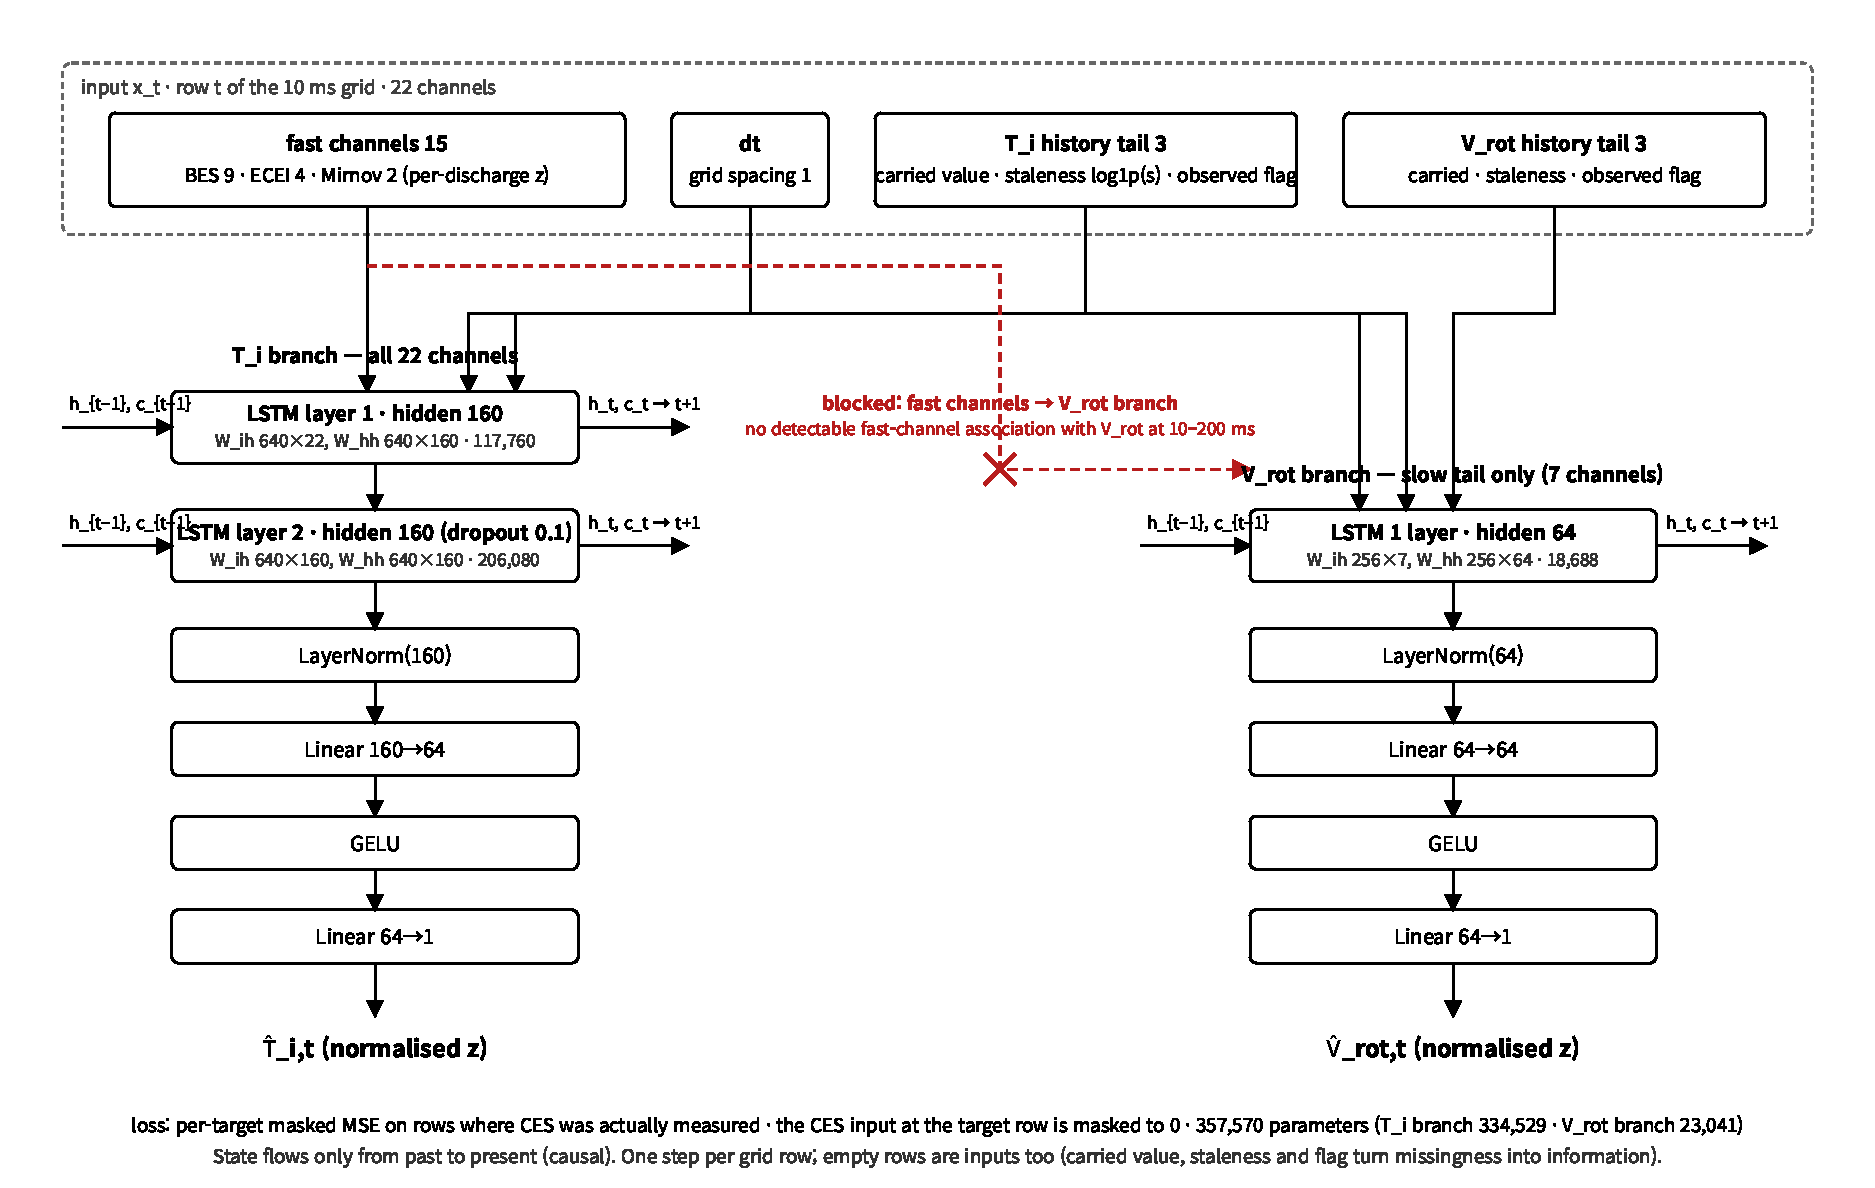
\includegraphics[width=0.8\textwidth]{fig_arch_seq_v2}
  \caption{\seqv{} for one grid row $t$. 22 inputs (15 fast, per-discharge $z$
  (whole-discharge statistics); $\Delta t$; per target carried value, staleness,
  observed flag) feed two LSTMs that run forward in time. The \Ti{}
  branch reads all 22 (2 layers, 160 units), the \Vrot{} branch only the seven slow
  channels (1 layer, 64 units); each ends in LayerNorm and Linear--GELU--Linear. The
  dashed red path from the fast channels to \Vrot{} does not exist by construction.
  357{,}570 parameters.}
  \label{fig:arch}
\end{figure*}

\seqv{} keeps every input-complete row of a contiguous segment, labelled or not, as
context, because the fast diagnostics have no gaps (Fig.~\ref{fig:arch}). Each step
carries 22 channels; every CES-derived input uses rows before $t$ only, while the 15
fast channels are standardized with the discharge's own mean and variance, an offline
step. The CES-derived channels are $\log(1{+}\Delta t_\mathrm{prev})$ and per target
the last observed value carried forward from rows $<t$, $\log(1{+}\text{staleness})$
and a has-any-past-observation flag. The \Ti{} branch reads all of them; the \Vrot{}
branch reads only the seven non-fast channels---the implementation
of~\S\ref{sec:model:physics}. Because the split is at the encoder, no shared recurrent
state carries fast information into the \Vrot{} head. Outputs are normalized
$[\Ti,\Vrot]$ per row, trained with~\eqref{eq:loss} over every labelled row (AdamW,
$\eta=10^{-3}$, weight decay $10^{-4}$, batch 16 segments, clipping 1.0, early stopping
with a 30-epoch cap). Splits are file-level, normalization of every other channel is
train-file-only, and the target row never enters the input. Under this protocol the
cost of a causal (training-statistics) standardization is not measured; under an
earlier protocol without the fit-failure cut, that variant kept a \Ti{} skill over
PCHIP of $+0.22$ to $+0.30$ with intervals excluding zero on 4/4 splits. Truncating the
backbone's own context costs $-0.066$ at 20\,ms and saturates at 50\,ms: the past
reaches the \Ti{} output through the carried CES value and about 50\,ms of
fast-channel context.

\paragraph{Windowed control and the gate.} The control (201{,}258 parameters), which
runs without per-discharge standardization, encodes each modality with its own
time-aware 1-D CNN over the $W{=}2$ preceding rows and reads the CES history with a
bidirectional GRU pooled by one multi-head attention readout per target, hard-masked so
that attention mass lands only on rows where that target was measured; its \Vrot{} head
also fuses history and time only. The full-grid framing was adopted over it by a
pre-registered four-condition gate on a $4\times4$ grid of split $\times$
initialisation seeds: paired \Ti{} skill positive on 16/16 runs, pooled $+0.081$
$[+0.067, +0.096]$. The control's skill over the causal GP is $+0.041$ (interval
including zero on 3/4 splits, cut).

\paragraph{Cost.} A stateful step costs 0.97\,ms median and 1.49\,ms at p99 on CPU;
deployment needs causal standardization.

\subsection{A 20-parameter surrogate of the \texorpdfstring{\Ti{}}{Ti} branch}
\label{sec:model:eq}
A pre-registered readout of the thirty frozen \seqv{} checkpoints found that weight
magnitude carries no stable information (first-layer column norms are flat across the
fifteen fast channels and per-channel ranks do not reproduce across splits), whereas
the input--output response does: the \Ti{} output is an exponentially weighted average
of past observed \Ti{} plus a same-instant response to the fast channels, with a
forget-gate memory of 1.3 grid steps. A frozen-row readout passed its registered bar, but a first trained
increment form fell below the registered 0.70 bar; the backbone's Jacobian on the test
rows then suggested Eq.~\eqref{eq:b28h}: a ${\approx}100$\,ms high-pass fast-channel
response (current value minus the preceding ten-step mean) with gain flat to $2\sigma$
and switched off beyond $3\sigma$. Because it was read on the test rows of the same four
splits on which the form is scored, the retention is post hoc. The corrected form,
trained from scratch under the identical protocol, is
\begin{gather}
  \hat y_t = m_t + \sum_{c=1}^{15} a_c\, d_{c,t}\,
     \sigma\!\Bigl(\frac{\theta-|d_{c,t}|}{0.5}\Bigr) + b_0,
  \label{eq:b28h}\\
  d_{c,t} = x_{c,t} - \overline{x}_{c,\,t-10..t-1},
  \nonumber\\
  m_t = m_{t-1} + K(s)\,(y^\mathrm{obs} - m_{t-1}),
  \nonumber\\
  K(s) = K_\infty + (K_0 - K_\infty)\,e^{-s/s_K},
  \label{eq:gain}
\end{gather}
where $m_t$ is updated only when a new \Ti{} measurement arrives, $s$ is the gap since
the previous one, and $\sigma(\cdot)$ is the logistic function; $d_{c,t}$ and $\theta$
are in per-discharge standard deviations (offline normalization). The first observation
of a segment is taken whole ($K=1$). Its 20 parameters
are three gain constants, one gain $a_c$ per fast channel, the threshold $\theta$ and
the offset $b_0$. Across the four cut splits the learned values are
$K_0 = 0.27$--$0.30$ for a fresh measurement, $K_\infty = 0.48$--$0.53$ after a long
gap, transition $s_K = 39$--$47$\,ms, $\theta = 2.9$--$3.0\sigma$,
$\sum a_{\mathrm{BES}} = +48$ to $+53$ and $\sum a_{\mathrm{ECEI}} = +44$ to $+50$\,eV
per $\sigma$. Read as a filter: a Kalman-like observation update that trusts a new CES
sample more the longer it has waited, plus a linear response to each fast channel's
departure from its 100\,ms baseline that rejects outliers beyond $3\sigma$. Since
$d_{c,t}$ is invariant to the per-discharge mean, the surrogate's offline dependence is
through the per-discharge $\sigma$ only. Its retention is in \S\ref{sec:res:eq}.

% =========================================================================
\section{Evaluation protocol}
\label{sec:eval}

\paragraph{Metric and baselines.} Errors are computed per target in physical units,
and the primary score is $\skillp = 1 - \mathrm{MSE}_{\mathrm{model}}/\mathrm{MSE}_{\mathrm{PCHIP}}$
(0 = equal error). Every arm is scored on the identical (file, row) set. Persistence,
a running mean and two-point extrapolation read only the past; linear, PCHIP and an
offline GP (Matérn-3/2 + white noise, nearest 16+16 neighbours, per-sample
marginal-likelihood selection) read the future; the causal GP is the same GP on the 16
past neighbours. Where no future neighbour exists the interpolant predicts persistence
(0.2\% of scored \Ti{} rows and 0.3--0.5\% of scored \Vrot{} rows).

\paragraph{Splits and pre-registration.} Files are split train/val/test with four
seeds (42, 1, 7, 123). Test files were reserved before the architecture search, but
the adoption of the sequence backbone, of per-discharge standardization and the
surrogate's form used results on the same four test splits; the repeated
cross-validation re-partitions the same 639 discharges. The canonical test set holds
32{,}589 \Ti{} rows over 96 shots and 10{,}463 \Vrot{} rows over 60 shots (cut).
``Pre-registered'' means the hypotheses, decision rules and numerical predictions of a
batch were committed to the repository before it was run; there is no third-party
registry.

\paragraph{Intervals.} Per-sample paired squared-error differences are aggregated by
shot and whole shots resampled (10{,}000 resamples); a result is reported with whether
its 95\% interval excludes zero. With four splits, each split's value is given with its own interval, together with the range and the number of splits whose interval excludes zero, rather than a mean $\pm$ standard deviation of four numbers~\citep{Weissgerber2015Beyond,Agarwal2021Deep}. Because the four splits share most of their training
discharges, the backbone was re-run as shot-level repeated 5-fold cross-validation on
639 discharges (ten repeats, 100 runs, every discharge tested once per repeat).
\emph{Fold-level}: the Nadeau--Bengio interval
$\bar S \pm t_{0.975,n-1}\sqrt{(1/n + n_{\mathrm{test}}/n_{\mathrm{train}})\,s^2}$~\citep{Nadeau2003Inference}.
\emph{Pooled}: each repeat's five test folds concatenated into one skill, with a
two-level bootstrap that draws a repeat and then resamples its discharges. The repeated
cross-validation was registered with the fold-level interval as its deciding readout;
for \Vrot{} against PCHIP it included zero. A pooled readout was then computed post
hoc, and eight new repeats were registered with the pooled two-level readout as
deciding before any of them ran. That interval conditions on the trained models and
does not carry the correlation between overlapping training sets; the fold-level
interval does.

% =========================================================================
\section{Results}
\label{sec:results}

\subsection{RMSE ladder}
\label{sec:res:ladder}
Table~\ref{tab:ladder} gives the physical-unit RMSE on the canonical test split. Among
the methods that do not read future CES values, \seqv{} has the lowest RMSE, 4\% (\Ti)
below the causal GP, and it is also below linear and PCHIP
interpolation. The offline GP, which averages noisy anchors, is the one arm with a
lower \Ti{} RMSE (153.8 vs.\ 157.8). Linear interpolation is the stronger offline
interpolant here: per split, the \Ti{} skill over it is $+0.136$ to $+0.226$ (cut) and
$+0.209$ to $+0.288$ (inclusive), the interval excluding zero on 4/4 splits in both
populations, 0.01--0.05 below the skill over PCHIP; for \Vrot{} it excludes zero on
1/4 splits in each population.

\begin{table}[t]
  \centering
  \caption{RMSE, seed-42 test split, cut population, genuine measurements only
  ($n = 32{,}589$ \Ti{}, $10{,}463$ \Vrot{}). Blocks: past CES only; past CES + fast
  channels, standardized per discharge (offline step; the windowed control uses
  training statistics); past + future CES. Inclusive:
  \seqv{} 363.0 / 23.7, PCHIP 412.4 / 30.2, causal GP 394.6 / 28.8, persistence
  478.0 / 33.4. \Vrot{} RMSEs are without the fit-failure rule of
  \S\ref{sec:res:headline}; under it (2 rows dropped on this split) the backbone's
  \Vrot{} skill is $+0.088$ $[+0.019, +0.145]$ over the causal GP, $+0.215$
  $[+0.071, +0.289]$ over PCHIP and $+0.329$ $[+0.265, +0.368]$ over persistence.}
  \label{tab:ladder}
  \footnotesize
  \setlength{\tabcolsep}{3.3pt}
  \begin{tabular}{llrr}
    \toprule
    Arm & Information & \Ti{} (eV) & \Vrot{} (km/s) \\
    \midrule
    Causal GP & past 16 CES & 164.3 & 28.8 \\
    Running mean & past CES & 169.2 & -- \\
    Persistence & last observed CES & 197.2 & 33.4 \\
    Two-point extrap. & past 2 CES & 472.2 & 51.0 \\
    \midrule
    \textbf{\seqv{}} & fast + past CES, segment & \textbf{157.8} & \textbf{23.6} \\
    20-param. surrogate$^{a}$ & fast + past CES & 162.3 & -- \\
    Windowed control & fast + 2 rows past CES & 169.2 & 26.1 \\
    \midrule
    GP (offline) & past + future CES & 153.8 & 24.7 \\
    Linear interp. & past + future CES & 169.8 & 29.0 \\
    PCHIP & past + future CES & 173.6 & 30.2 \\
    \bottomrule
  \end{tabular}

  \smallskip\raggedright\scriptsize $^{a}$An interpretation of the backbone, not a
  standalone-estimator claim; paired skill over the causal GP on this split $+0.024$
  $[-0.012, +0.057]$.
\end{table}

\subsection{Headline and replicate}
\label{sec:res:headline}

\begin{table*}[t]
  \centering
  \caption{Skill of \seqv{} against each comparator. \emph{Four splits}: range of the
  per-split skill over seeds 42/1/7/123 with the number of splits whose
  shot-clustered 95\% CI excludes zero. \emph{Fold-level}: Nadeau--Bengio 95\% interval
  over 50 folds of repeated 5-fold CV, with the number of folds whose own CI excludes
  zero; this was the deciding readout as first registered. \emph{Pooled}: median and
  two-level bootstrap 95\% interval over eight re-partitions of the same 639
  discharges, registered as deciding before those repeats ran. Bold = interval excludes
  zero. The four-split offline GP entries pool both populations. \Vrot{} rows are the
  registered readout without the fit-failure rule of \S\ref{sec:res:headline}.}
  \label{tab:headline}
  \footnotesize
  \setlength{\tabcolsep}{3pt}
  \resizebox{\textwidth}{!}{%
  \begin{tabular}{llcccccc}
    \toprule
    & & \multicolumn{2}{c}{Four splits} & \multicolumn{2}{c}{Fold-level (repeated 5-fold)} & \multicolumn{2}{c}{Pooled (two-level)} \\
    \cmidrule(lr){3-4}\cmidrule(lr){5-6}\cmidrule(lr){7-8}
    Target & vs. & cut & inclusive & cut & inclusive & cut & inclusive \\
    \midrule
    \multirow{4}{*}{\Ti{}}
      & PCHIP       & $+0.174$ to $+0.264$ (\textbf{4/4}) & $+0.225$ to $+0.316$ (\textbf{4/4}) & $\mathbf{[+0.186, +0.253]}$ (50/50) & $\mathbf{[+0.188, +0.307]}$ (46/50) & $+0.221$ $\mathbf{[+0.188, +0.248]}$ & $+0.248$ $\mathbf{[+0.192, +0.294]}$ \\
      & persistence & $+0.360$ to $+0.415$ (\textbf{4/4}) & $+0.406$ to $+0.459$ (\textbf{4/4}) & $\mathbf{[+0.368, +0.410]}$ (50/50) & $\mathbf{[+0.361, +0.445]}$ (50/50) & $+0.391$ $\mathbf{[+0.369, +0.408]}$ & $+0.404$ $\mathbf{[+0.364, +0.438]}$ \\
      & causal GP   & $+0.078$ to $+0.138$ (\textbf{4/4}) & $+0.123$ to $+0.169$ (\textbf{4/4}) & $\mathbf{[+0.084, +0.138]}$ (47/50) & $\mathbf{[+0.067, +0.170]}$ (40/50) & $+0.113$ $\mathbf{[+0.085, +0.132]}$ & $+0.118$ $\mathbf{[+0.076, +0.157]}$ \\
      & offline GP  & \multicolumn{2}{c}{$-0.05$ to $+0.11$ (CI includes 0 on 7/8)} & $[-0.044, +0.020]$ (1/50) & $[-0.026, +0.094]$ (12/50) & $-0.010$ $[-0.043, +0.014]$ & $+0.035$ $[-0.017, +0.075]$ \\
    \midrule
    \multirow{4}{*}{\Vrot{}}
      & PCHIP       & $+0.135$ to $+0.390$ (1/4) & $+0.132$ to $+0.384$ (2/4) & $[-0.021, +0.405]$ (15/50) & $[-0.053, +0.391]$ (11/50) & $+0.313$ $\mathbf{[+0.072, +0.701]}$ & $+0.319$ $\mathbf{[+0.046, +0.683]}$ \\
      & persistence & \multicolumn{2}{c}{$+0.30$ to $+0.50$ (3/4 in each)} & $\mathbf{[+0.190, +0.601]}$ (42/50) & $\mathbf{[+0.159, +0.587]}$ (38/50) & $+0.451$ $\mathbf{[+0.277, +0.763]}$ & $+0.451$ $\mathbf{[+0.139, +0.747]}$ \\
      & causal GP   & $+0.020$ to $+0.331$ (2/4) & $+0.018$ to $+0.324$ (2/4) & $[-0.060, +0.512]$ (11/50) & $[-0.096, +0.502]$ (10/50) & $+0.361$ $\mathbf{[+0.045, +0.701]}$ & $+0.357$ $\mathbf{[+0.023, +0.683]}$ \\
      & offline GP  & \multicolumn{2}{c}{$-0.07$ to $+0.09$ (CI includes 0 on 7/8)} & $[-0.234, +0.312]$ (0/50) & $[-0.268, +0.300]$ (0/50) & $+0.262$ $[-0.119, +0.635]$ & $+0.251$ $[-0.139, +0.609]$ \\
    \bottomrule
  \end{tabular}}
\end{table*}

\paragraph{\Ti{}.} Table~\ref{tab:headline}: $\skillp = +0.17$ to $+0.26$ (cut) and
$+0.23$ to $+0.32$ (inclusive), every shot-clustered interval excluding zero on all
four splits; over the causal GP $+0.08$ to $+0.17$ and over persistence $+0.36$ to
$+0.46$, both excluding zero on 8/8 population--split cells. Against the offline GP
the paired skill is $-0.05$ to $+0.11$ with the interval including zero on 7/8 cells:
the margin is over interpolants and causal smoothers, not over every offline smoother.
The replicate reproduces every verdict: vs.\ PCHIP the fold-level interval is
$[+0.19, +0.25]$ (cut) and $[+0.19, +0.31]$ (inclusive). The skill is not
confined to adjacent history: beyond $\Delta t > 15$\,ms since the last observation it
is $+0.268$ (cut) and $+0.206$ (inclusive) over PCHIP, both intervals excluding zero.

\paragraph{\Vrot{}.} Point estimates are positive on every split, but the four-split
interval over PCHIP excludes zero on 1/4 (cut) and 2/4 (inclusive) splits, and the
fold-level interval includes zero ($[-0.02, +0.41]$ cut). The pooled readout over
eight re-partitions of the same 639 discharges excludes zero over PCHIP, persistence
and the causal GP (Table~\ref{tab:headline}), but that margin over PCHIP rests on fit
failures. A rule that removes, from every arm, the rows whose target, persistence
anchor or PCHIP anchor exceeds $|\Vrot| = 1{,}000$\,km/s drops 36--41 of about 71{,}700
rows per repeat (0.05\%), which carry 63--78\% of PCHIP's squared error (cut). This
rule was set during review, after the share carried by these rows was known; it is
applied when scoring only, so the history inputs still contain the fit failures and no
model was retrained. Under this rule the pooled skill over PCHIP is $+0.092$
$[+0.0003, +0.170]$ (cut) and $+0.090$ $[-0.010, +0.177]$ (inclusive), and it includes
zero in both populations at thresholds of 500 and 2{,}000\,km/s, so a \Vrot{} margin
over PCHIP is not established. Over persistence it is $+0.265$ $[+0.198, +0.326]$ (cut)
and $+0.257$ $[+0.183, +0.323]$ (inclusive), per split 4/4 in both populations at 500
and 1{,}000\,km/s and 3/4 at 2{,}000\,km/s. Over the causal GP it is $+0.151$
$[+0.038, +0.290]$ and $+0.132$ $[+0.026, +0.267]$, excluding zero at all three
thresholds; per split it is $+0.057$ to $+0.131$ (cut, interval excluding zero on 1/4)
and $+0.053$ to $+0.143$ (inclusive, 2/4), every point estimate positive; a fold-level
interval under the rule was not computed. Against the offline GP the history-only
estimate has $-0.073$ $[-0.162, +0.005]$ (cut, including zero) and $-0.087$
$[-0.174, -0.008]$ (inclusive). The \Vrot{} margin is established against persistence
on every split; against the causal GP only in the pooled readout.

\paragraph{Why inclusive numbers are higher.} Every arm scores higher against PCHIP
without the cut (backbone mean $+0.268$ vs.\ $+0.236$) because spikes poison the
interpolation anchors, which a learned model can discount; this is why neither
population is quoted alone.

\paragraph{Two stress tests.} \emph{Missing-not-at-random:} reweighting the scored
rows onto the covariate distribution ($\Delta t$ $\times$ local activity) of the
genuinely missing, in-domain rows---53.6--67.0\% (cut) and 54.1--67.7\% (inclusive) of
missing \Ti{} rows---gives \Ti{} skill over PCHIP $+0.14$ to $+0.28$ with intervals
excluding zero on 2/4 cut and 4/4 inclusive splits, and over persistence $+0.28$ to
$+0.44$ with intervals excluding zero on 8/8 cells (missing \Vrot{} rows are only
4--6\% in-domain, and we draw nothing from them). \emph{Campaign shift:} with a strictly
temporal split (train 416 shots, val 128, test the 97 latest), \seqv{} keeps $+0.17$
to $+0.20$ over PCHIP and $+0.11$ to $+0.16$ over the causal GP, intervals excluding
zero on 4/4 initialisations in both populations, where the windowed control keeps
$-0.001$ to $+0.091$ (2/4 cut, 0/4 inclusive); for \Vrot{} the skill is $+0.19$ to
$+0.23$ over PCHIP (intervals including zero on 4/4) and $+0.33$ over persistence
(4/4, cut). The fast diagnostics drift 1.22$\sigma$ (BES) and 0.53$\sigma$ (ECEI)
between periods against 0.115$\sigma$ for the targets. Per-discharge standardization
was adopted after the windowed control failed this split, and it uses whole-discharge
statistics, so this is not an independent test of a deployable estimator.

\subsection{\texorpdfstring{The \Ti$\leftrightarrow$\Vrot{} asymmetry}{The Ti-Vrot asymmetry}}
\label{sec:res:asym}
Corrected for target noise, the correlation of fast-channel and \Vrot{} increments has
a 95\% bound $|r| \leq 0.044$ over every lag (0--200\,ms) and window (10--200\,ms),
against a \Ti{} lower bound of at least $+0.127$ at lag 0 for every window 10--200\,ms; this
bounds a linear association and does not prove its absence (BES at 100--200\,ms gives
$r \approx +0.01$ with an interval excluding zero). Zeroing one input group at
evaluation time on the windowed control (Table~\ref{tab:ablation}) feeds inputs the
control never saw; the No-fast cut row ($-0.125$) lies below a CES-only running mean
($+0.05$ to $+0.17$ over PCHIP), so the table measures sensitivity to
out-of-distribution inputs, not a group's contribution. A retrained history-only
backbone has not been run. A validation-tuned running mean sits at $-0.060$ to $+0.003$
against the causal GP, so the backbone's margin over the causal GP is close to its
margin over that running mean ($+0.113$ to $+0.137$, cut, 4/4; inclusive $+0.061$ to
$+0.140$, 4/4); event rows concentrate it (top-10\% $|d\mathrm{ECEI}|$ rows, seeds
42/1: backbone $+0.116$/$+0.269$ over PCHIP against $-0.011$/$+0.088$ for the running
mean plus a linear fast-channel term). In the inclusive population the windowed
control without fast channels still has $+0.15$ to $+0.23$ over PCHIP, a
spike-robustness component. For \Vrot{} the control's output is bit-identical without
the fast channels, a consequence of the routing; the evidence for the routing is
\S\ref{sec:model:physics}, the bound above and the two routes below.

\begin{table}[t]
  \centering
  \caption{Evaluation-time input sensitivity of the windowed control (no retraining):
  $\skillp$ for \Ti{} (4-split mean) and the paired change against the full model
  ($^{*}$ = significant splits). Zeroed inputs are out of distribution for the control,
  so the rows measure sensitivity, not a group's contribution.}
  \label{tab:ablation}
  \footnotesize
  \setlength{\tabcolsep}{2.5pt}
  \resizebox{\linewidth}{!}{%
  \begin{tabular}{lcc}
    \toprule
    Inputs & cut & inclusive \\
    \midrule
    Full & $+0.173$ & $+0.238$ \\
    No fast & $-0.125$; $-0.25$ to $-0.42$ (4/4$^{*}$) & $+0.201$; $-0.03$ to $-0.09$ (2/4$^{*}$) \\
    No history & $-2.11$ & $-1.16$ \\
    \bottomrule
  \end{tabular}}
\end{table}

\paragraph{Two routes to rotation information.} \emph{Mirnov:} on 24 of 24
coils checked against the raw 2\,MHz stream, the 100\,Hz value equals a single raw
sample at the grid time (lag 0), a point snapshot, so the kHz mode rotation is aliased
away. \emph{Beam
torque:} no torque channel exists, so beam torque is untested here. The statement is
scoped to standard CES at 10\,ms at the $R = 2.198$\,m chord; edge rotation inside an
ELM cycle~\citep{Viezzer2020Dynamics} is a different measurement.

\subsection{Surrogate retention}
\label{sec:res:eq}
Trained from scratch under the identical protocol, the 20-parameter surrogate
filter~\eqref{eq:b28h}--\eqref{eq:gain} keeps \textbf{72--78\%} of the backbone's
PCHIP-relative skill and 87--90\% of its persistence-relative skill on 4/4 cut splits,
above the registered bar of 0.70; measured against the causal GP it keeps 0.31 to 0.50
of the backbone's skill (cut, point estimates). It sits above the first increment form
by a paired $+0.034$ to $+0.042$ with intervals above zero on 4/4 splits. Because the
Jacobian was read on the same test rows, this retention is post hoc. The remaining
22--28\% is the network's nonlinear event handling, which the three forms tried here do
not reproduce. As a standalone estimator (cut) the surrogate has skill $+0.13$ to
$+0.21$ over PCHIP (4/4 splits), $+0.02$ to $+0.07$ over the causal GP (interval
excluding zero on 2/4), and is below the offline GP on 4/4. These are measurements of
the model; the headline numbers remain the backbone's. The bands are read from the cut population only: in
the inclusive population the surrogate keeps 0.43--0.81 of the PCHIP-relative skill and
its BES gain changes sign under the fit-failure spikes.

\subsection{Mean and median: a dual readout}
\label{sec:res:dual}
An MSE skill is decided by few rows: the backbone's top 1\% of \Ti{} squared-error
rows carry 48\% (cut) and 83\% (inclusive) of the total. On a typical row the backbone
carries its anchor: its median absolute \Ti{} error of 47.2\,eV is close to persistence's
46.1\,eV and the target's own 10\,ms scatter of 46.4\,eV, while PCHIP reaches 39.4\,eV
by averaging with the future neighbour (median-AE skill $-0.198$
$[-0.259, -0.135]$, win rate 0.48); the error ratio model/PCHIP falls below 1 only in
the upper error quartile. For \Vrot{} the backbone's median row is worse than
persistence (4.3 vs.\ 3.7\,km/s; median-AE skill vs.\ PCHIP $-0.488$ cut and $-0.518$
inclusive, interval below zero on 4/4 splits): its aggregate skill is a bulk deficit
offset by a tail gain. Under a symmetric 1\% trim and a Huber loss at the noise bound
the \Ti{} skill over PCHIP stays $+0.210$ and $+0.156$ (cut, both intervals excluding
zero); the inclusive trimmed skill is $+0.057$ (interval including zero). A separate,
pre-registered scalar hold-or-jump filter run causally on the CES history (Student-$t$
measurement noise at the 10\,ms bulk scatter) has a \Ti{} median absolute error
0.906--0.920$\times$ persistence (8/8 split--population cells excluding 1); for \Vrot{}
its ratio is 0.94--1.00$\times$ (interval including 1 on 3/4 splits, also when fitted
on the training files). The 10\,ms scatter is
consistent with independent Gaussian line-fit errors: the ratio of relative \Ti{} to
\Vrot{} scatter is $\sqrt2$ on 8/8 cells (1.395--1.532), while the $\sqrt{T_i}$ scaling
expected of photon statistics was not observed (slope 0.09--0.23 against 0.5); between
labels the median-optimal point is the last value. The filter's MSE skill against the
backbone is $-0.06$ to $-0.52$, because event rows stay late.

% =========================================================================
\section{Limitations and conclusion}
\label{sec:conclusion}

\paragraph{Limitations.} The aggregate skill is a tail statistic; typical rows are not
improved over PCHIP. The fast channels are standardized with whole-discharge
statistics, an offline step, so a deployable variant is untested under this protocol;
under an earlier protocol a training-statistics variant kept $+0.22$ to $+0.30$ over
PCHIP (4/4) but was not scored against the causal GP. Two choices were made post hoc:
the surrogate's form (chosen on the scored splits; its retention holds in the cut
population only, inclusive 0.43--0.81) and the 1{,}000\,km/s \Vrot{} rule. The unit of
replication is the shot; the reweighting reaches only 4--6\% of missing \Vrot{} rows.
Everything is one chord, one device and one campaign.

\paragraph{Conclusion.} For an estimate that cannot wait for the next CES exposure, the
full-input causal estimator, with fast channels standardized per discharge, has \Ti{} skill
$+0.113$ $[+0.085, +0.132]$ over the CES-only causal GP (cut); the fast-channel share is not isolated, and against an
offline noise-aware smoother of both neighbours the skill interval includes zero.
\Vrot{} at this chord is estimated from its own history; its margin is established
against persistence on every split and against the causal GP only in the pooled
readout, and its 10\,ms scatter is consistent with Gaussian line-fit errors. Code and evaluation artifacts:
\url{https://github.com/iseungsang01/ml-intern-revision}.

\paragraph{Acknowledgments and data use.} [To be completed by the author: data
provider and KFE permission for the KSTAR 2022 CES, BES, ECEI and Mirnov data.]

{\small
\bibliographystyle{unsrtnat}
\bibliography{../refs}
}

\end{document}
